\chapter{METODOLOGÍA DE LA INVESTIGACIÓN}
\section{Diseño de la investigación}

En este segmento del documento se explica cual fue el tipo y enfoque del trabajo de
investigación, al igual que la población y la muestra. 

\subsection{Tipo de Investigación}
El diseño del presente trabajo de investigación es de tipo no experimental, ya que no se manipulan las variables independientes y se observa su relación en el contexto de la implementación de un modelo de traducción de lenguaje de señas utilizando técnicas de Deep Learning. La etapa inicial del trabajo involucra el análisis de vídeos de lenguaje de señas, los cuales serán procesados mediante técnicas de Deep Learning. \\

El nivel del presente trabajo de investigación es explicativo, dado que se enfoca en la implementación de un modelo de traducción de lenguaje de señas utilizando Deep Learning para personas con discapacidad del habla. El objetivo es determinar cómo se puede lograr la traducción efectiva del lenguaje de señas a texto y viceversa, estableciendo una relación entre los gestos y movimientos específicos del lenguaje de señas y su correspondencia con el texto escrito. \\



\subsection{Enfoque de Investigación}

El enfoque del presente trabajo de investigación es cuantitativo, dado que se basa en la utilización de instrumentos para la identificación y medición del lenguaje de señas a través de técnicas de visión computacional. Estas técnicas proporcionarán resultados numéricos que, tras un análisis estadístico, servirán como entrada para implementar modelos de Deep Learning. 



\section{Población y muestra}

\begin{table}[h!]
	\centering
	\caption{Descripción del Estudio}
	\begin{tabular}{|>{\raggedright\arraybackslash}m{3cm}|>{\raggedright\arraybackslash}m{10cm}|}
		\hline
		\textbf{Categoría} & \textbf{Descripción} \\ \hline
		\textbf{Población} & Personas con discapacidades del habla y del escucha. \\ \hline
		\textbf{Muestra} & 
		\begin{itemize}
			\item 260 vídeos MP4 de diálogos en lenguaje de señas extraídas de Universidad Pontificia Universidad Católica del Perú.
			\item 355 vídeos MP4 de narración de historias en lenguaje de señas extraídas de Universidad Pontificia Universidad Católica del Perú.
			\item 103 vídeos MP4 de nombres, estados y acciones en lenguaje de señas extraídas de Universidad Pontificia Universidad Católica del Perú.
		\end{itemize}
		\\ \hline
		\textbf{Unidad de análisis} & Un vídeo de una persona comunicándose con lenguaje de señas \\ \hline
	\end{tabular}
\end{table}


\section{Operacionalización de Variables}

\begin{table}[h!]
	\centering
	\caption{Operacionalización de Variables}
	\begin{tabular}{|>{\raggedright\arraybackslash}m{4cm}|>{\raggedright\arraybackslash}m{4cm}|>{\raggedright\arraybackslash}m{4cm}|>{\raggedright\arraybackslash}m{4cm}|}
		\hline
		\textbf{Variable} & \textbf{Dimensión} & \textbf{Indicador} & \textbf{Cálculo} \\ \hline
		\textbf{Independiente: Modelo Deep Learning} 
		& Base de datos & Volumen de datos & Cantidad de videos MP4\\ \cline{2-4}
		
		\textbf{Dependiente: Traducción de Lenguaje de señas peruano para personas con discapacidades del habla} 
		& Indicadores de rendimiento de modelo & Precisión, recall, F1-score & Fórmulas \\ \hline
	\end{tabular}
\end{table}

\section{Técnicas de recolección}
	
	La base de datos se compone de vídeos en formato MP4 proporcionados por la Universidad Pontificia Universidad Católica del Perú. Estos vídeos fueron seleccionados por su relevancia y calidad para el estudio del lenguaje de señas. Los videos MP4 contienen diálogos, narraciones de historias, y nombres, estados y acciones en lenguaje de señas.


\section{Técnicas para el procesamiento y análisis de la información}

\subsection{Metodología de la implementación de la solución}

\subsubsection{Recolección de Datos}
La recolección de datos es una fase crítica en cualquier proyecto de Deep Learning. En esta tesis, se han recopilado un total de 718 vídeos MP4 de lenguaje de señas, extraídos de la Pontificia Universidad Católica del Perú. Los datos se dividen en tres categorías principales:
\begin{itemize}
	\item \textbf{260 vídeos MP4 de diálogos en lenguaje de señas}: Estos vídeos contienen conversaciones entre dos o más personas utilizando lenguaje de señas.
	\item \textbf{355 vídeos MP4 de narración de historias en lenguaje de señas}: En estos vídeos, las personas narran historias completas usando lenguaje de señas.
	\item \textbf{103 vídeos MP4 de nombres, estados y acciones en lenguaje de señas}: Estos vídeos muestran la señalización de nombres, estados emocionales y diversas acciones.
\end{itemize}

\subsubsection{Preprocesamiento de Datos}
El preprocesamiento de datos es una etapa esencial para preparar los datos brutos para ser utilizados por los modelos de Deep Learning. Las tareas de preprocesamiento incluyen:
\begin{itemize}
	\item \textbf{Extracción de Frames}: Se extraen frames de los vídeos a intervalos regulares para capturar las diferentes poses y movimientos de las manos.
	\item \textbf{Aumento de Datos}: Se aplican técnicas de aumento de datos, como rotación, escalado y traslación, para aumentar la variabilidad y robustez del conjunto de datos.
	\item \textbf{Etiquetado}: Cada frame o secuencia de frames se etiqueta con la correspondiente señal del lenguaje de señas que representa.
	\item \textbf{Normalización}: Los frames se normalizan para asegurarse de que todos los datos tengan el mismo formato y escala.
\end{itemize}

\subsubsection{Uso de Redes Neuronales Convolucionales (CNN)}
Las redes neuronales convolucionales (CNN) son efectivas para la tarea de reconocimiento de imágenes y, en este caso, para la identificación de señales en los frames extraídos de los vídeos. Las etapas clave incluyen:
\begin{itemize}
	\item \textbf{Diseño de la Arquitectura CNN}: Se diseña una arquitectura de CNN adecuada para la tarea, con capas convolucionales, de pooling y totalmente conectadas.
	\item \textbf{Entrenamiento}: La CNN se entrena utilizando los datos preprocesados, ajustando los pesos de la red para minimizar el error en la predicción de las señales.
	\item \textbf{Validación}: Se valida el rendimiento de la CNN utilizando un conjunto de datos de validación separado, ajustando los hiperparámetros según sea necesario.
\end{itemize}

\subsubsection{Integración de LSTM}
Las redes neuronales de memoria a largo plazo (LSTM) son ideales para manejar secuencias de datos y capturar dependencias temporales. En esta fase:
\begin{itemize}
	\item \textbf{Extracción de Secuencias}: Se crean secuencias de frames para capturar el movimiento y la continuidad de las señales.
	\item \textbf{Diseño de la Arquitectura LSTM}: Se diseña una arquitectura LSTM que pueda procesar las secuencias de frames y capturar las dependencias temporales entre ellos.
	\item \textbf{Entrenamiento del Modelo}: El modelo LSTM se entrena para aprender las transiciones y la continuidad de las señales en las secuencias de frames.
	\item \textbf{Combinación con CNN}: La salida de la CNN se combina con la LSTM para mejorar la precisión en la predicción de señales.
\end{itemize}

\subsubsection{Evaluación del Modelo}
La evaluación del modelo es crucial para determinar su eficacia y áreas de mejora. Las actividades incluyen:
\begin{itemize}
	\item \textbf{Métricas de Evaluación}: Se utilizarán métricas como Recall, F1-Score y Accuracy para evaluar el rendimiento del modelo.
	\item \textbf{Pruebas con Datos de Prueba}: Se prueba el modelo con un conjunto de datos de prueba que no se ha utilizado durante el entrenamiento para evaluar su rendimiento en datos no vistos.
	\item \textbf{Análisis de Errores}: Se realiza un análisis de errores para identificar patrones comunes en las predicciones incorrectas y mejorar el modelo.
	\item \textbf{Ajustes y Mejoras}: Basado en los resultados de la evaluación, se ajustan los hiperparámetros y se realizan mejoras en la arquitectura del modelo para aumentar su rendimiento.
\end{itemize}

\begin{figure}[h!]
	\centering
	\includegraphics[width=1\textwidth]{3/figures/Metodología.png}
	\caption{Metodología Iterativa}
	\label{fig:etiqueta_de_la_figura}
\end{figure}


\subsection{Metodología para la medición de resultados}

\subsection*{Accuracy}
El accuracy medirá la proporción de predicciones correctas sobre el total de predicciones realizadas por el modelo Deep Learning. Se utilizará para obtener una visión general del rendimiento del modelo.
\begin{equation}
	\text{Accuracy} = \frac{TP + TN}{TP + TN + FP + FN}
\end{equation}

\subsection*{Recall}
El Recall medirá la capacidad del modelo para identificar correctamente todas las instancias positivas.
\begin{equation}
	\text{Recall} = \frac{TP}{TP + FN}
\end{equation}

\subsection*{F1-Score}
Se utilizará en caso el modelo presente un desequilibrio entre las clases y se necesita un equilibrio tanto en el Accuracy como en el recall.
\begin{equation}
	\text{F1-Score} = 2 \cdot \frac{\text{Precision} \cdot \text{Recall}}{\text{Precision} + \text{Recall}}
\end{equation}


\section{Cronograma de actividades}
\begin{figure}[h!]
	\centering
	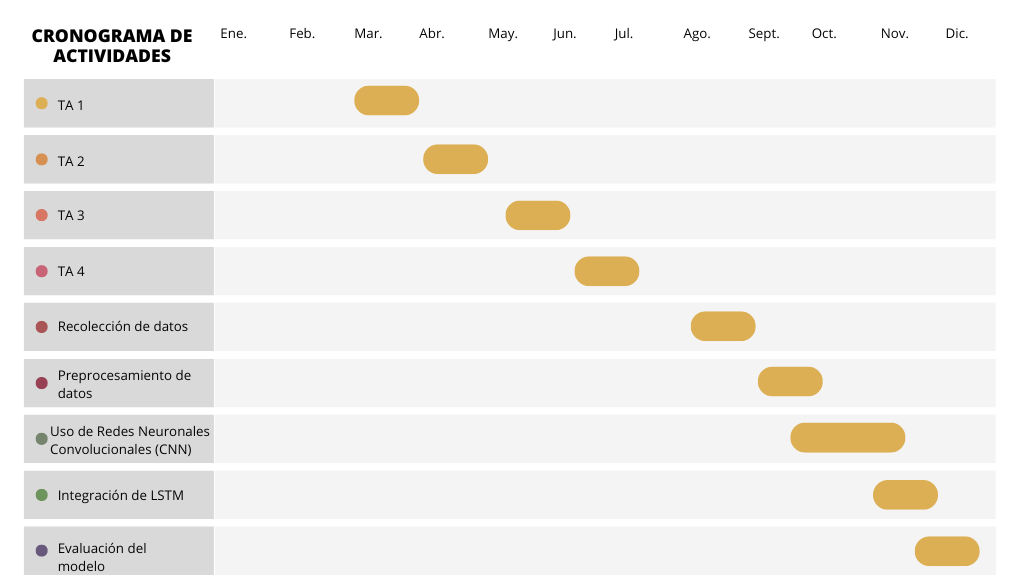
\includegraphics[width=1\textwidth]{3/figures/Actividades.png}
	\caption{Metodología Iterativa}
	\label{fig:etiqueta_de_la_figura}
\end{figure}
\section{Presupuesto}


\begin{table}[h!]
	\centering
	\caption{Presupuesto del Proyecto}
	\begin{tabular}{|>{\raggedright\arraybackslash}m{10cm}|>{\raggedright\arraybackslash}m{4cm}|}
		\hline
		\textbf{Item} & \textbf{Costo (Soles)} \\ \hline
		Laptop & 3500 \\ \hline
		Cámara & 250 \\ \hline
		\textbf{Total} & \textbf{3750} \\ \hline
	\end{tabular}
\end{table}